\section{Introduction} \label{sec:intro}
Elements heavier than hydrogen are produced through nuclear fusion. After Big Bang Nucleosynthesis, this only occurs in compact objects. The distribution of elemental abundances in the gas-phase of a galaxy is determined by a complicated combination of physical processes - stellar evolution and supernovae, gas accretion, galaxy mergers, gas outflows from stellar and AGN feedback, metal mixing and diffusion, etc.

By necessity, stars inherit the constituitive properties of the gas cloud from which they formed. Moreover, the surface abundance of stars do not change over time.\footnote{For the most part.} We therefore have the unique opportunity to examine the historical record of the gas-phase abundance of a galaxy by way of the distribution of the surface abundances of stars. Because the processes which give rise to this distribution are complex, there is almost certainly some structure in this distribution for every galaxy. However, it has only been definitively measured in the Milky Way.

The distribution of elemental abundances is a high dimensional space (\red{e.g. up to 8 billion elements by XYZ}). However, this space is highly degenerate, and so the effective number of dimensions is much smaller - even possibly compressed to just \FeH and age \citep{2019ApJ...883..177N}.

Two elements in particular have received particular interest - iron and $\alpha$-elements (elements produced through the $\alpha$-process, typically tracked with just Mg). Type Ia and Type II supernovae are the main contributors of elemental enrichment. Iron is broadly produced in both types, and so its abundance is a proxy for the total metallicity of a star. $\alpha$-elements, on the other hand, are mainly produced in Type II supernovae. The ratio of $\alpha$-elements to iron is then a measure of the relative contributions of Type Ia and II to the enrichment of a parcel of gas. It has therefore become common to compress the high-dimensional abundance space to the two dimensional \FeH-\alphaFe plane.

In this plane, it is now well-established that a significant bimodality exists in the Milky Way \red{cite a boatload}.





Elemental enrichment is accounted for in modern galaxy formation models, though the validity of the yield tables is suspect. It is not known if the yields (i.e., the amount of metals produced by the SN) used in such models are accurate. This issue is further compounded by the fact that the mixing of metals is unresolved and is sensitive to numerical choices (e.g., Eulerian codes being generally more diffusive than Lagrangian). To make matters even worse, the inflows and outflows of gas from galaxies is sensitive to the choices of the feedback model, which has a strong impact on a galaxy's elemental history.




The last\footnote{i.e., not ongoing} significant merger was between the
proto-Milky Way disk and the {\em Gaia}-Sausage-Enceladus (GSE)
(\textcolor{red}{spell check}) satellite galaxy. The stellar debris from this
merger constitutes $\sim50\%$ \textcolor{red}{check} of the inner ($r<?\,\kpc$)
stellar halo. It may have also led to a tilted, triaxial dark matter halo
(\textcolor{red}{cite}).

The GSE merger is often invoked (\textcolor{red}{cite}) to explain the observed
bimodality in the \textcolor{red}{alpha iron} abundance plane
(\textcolor{red}{cite}). Because GSE-mass galaxies are expected to have a lower
star formation efficiency than proto-Milky Way-mass galaxies
(\textcolor{red}{cite}), the gas from GSE should be relatively metal poor. The
gas from GSE thus dilutes the gas in the proto-Milky Way, ``resetting'' the
chemical abundance of the Milky Way.

However, it has also been claimed that the \textcolor{red}{alpha iron}
bimodality can be explained through secular processes. \textcolor{red}{Sentence
explaining the basic concept.} The argument is not that the GSE merger did not
happen, but rather that it is not {\it necessary} and might not even be {\it
sufficient} to explain the bimodality. Ongoing work to detect the bimodality in
external galaxies may shed further light on the topic (\textcolor{red}{cite}).

Investigating GSE-like mergers in cosmological simulations is a rich and active
area of research. Many mergers believed to be similar to the GSE merger have
been identified in the literature (\textcolor{red}{cite}). \textcolor{red}{Blah
blah argue blah blah. And also blah blah argues blah blah.}

While much has been learned from GSE-like mergers in cosmological simulations,
they are not conducive to controlled experiments. It is possible to change the
mass of satellites through genetic modification (\textcolor{red}{Pontzen}), and
the GSE analog can be removed entirely (\textcolor{red}{Cooke cite}). However,
to our knowledge, no method has been applied to change the orbital parameters of
such a merger. It is also somehwat unclear if the circumgalactic media of
proto-Milky Way mass galaxies at $z\sim2$ are properly simulated.

In this work, we present hydrodynamic simulations of a controlled merger between
a GSE analog and the $z\sim2$ proto-Milky Way. 

\begin{figure*}
  \centering
  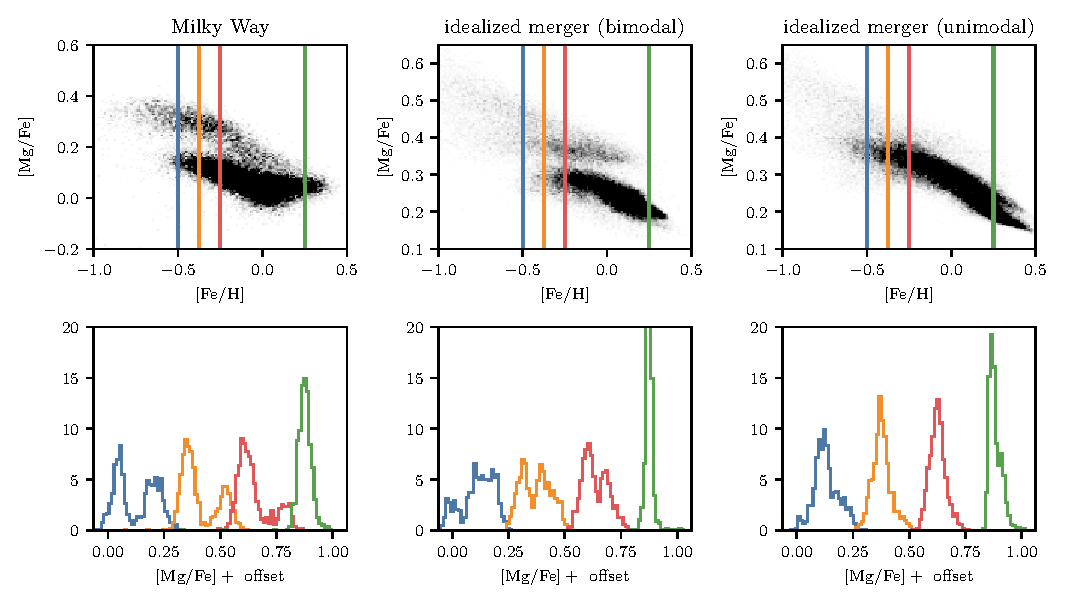
\includegraphics[width=\textwidth]{figure1.pdf}
  \caption{\textbf{The abundance bimodality seen in the Milky Way can be reproduced in some idealized merger simulations.} In the upper panels, we show the distribution of stars in the \MgFe-\FeH plane. The left panel shows the observed distribution in the Milky Way from ASPCAP \red{cite}, while the right two panels show two idealized merger simulations. The idealized merger simulations are nearly identical, except that the bimodal simulation has a starting radius of $129\,\kpc$, while the unimodal simulation has a starting radius of $142\,\kpc$. We emphasize that the labels ``unimodal'' and ``bimodal'' are of the \textit{outcome} of the simulation, and do not reflect a particular choice in the setup. The bottom panels show the distribution of \MgFe at fixed \FeH. The colors indicate the fixed \FeH values, which are $-0.5$, $-0.375$, $-0.25$, and $0.25$. The Milky Way (left panels) exhibits a strong bimodal distribution of \MgFe at various \FeH. The idealized merger simulation marked as bimodal (center panels) also exhibits a bimodal distribution of \MgFe, though the structure is not as strongly defined. The idealized merger simulation marked as unimodal exhibits only weak structure, if any at all.}
  \label{fig:fig1}
\end{figure*}